
\section{线丛与到射影空间的映射}

回想一下，\trAffine{}空间 $\mathbb{A}^n$ 曾有一个作为\trRepresentableFunctor{}的简短描述：映入 $\mathbb{A}^n$ 的（从 $X$ 出发的）映射，恰与「在 $X$ 上选取 $n$ 个函数」这份数据完全相同（\mbox{练习~7.6.E}(a)）。在本节中，我们会不经意间把\trProjectiveSpace{}也按同样的方式重新解释一遍。

设 $x_0$、$x_1$、$x_2$ 是 $\mathbb{P}^2_k$ 上的射影坐标。你能看出
\begin{equation*}\tag{15.2.0.1}\label{eq:cubic-map-morphism}
[x_0^3,\; x_0^2x_2,\; x_0x_1x_2+x_1^3,\; x_2^3]
\end{equation*}
如何给出一个\trMorphism{} $\mathbb{P}^2_k\to\mathbb{P}^3_k$ 吗？\eqref{eq:cubic-map-morphism} 的各个分量并不是函数，所以我们无法逐个地理解它们。但对 $\mathbb{P}^2_k$ 的任何一个「点」，它们的比值仍可以有意义。例如，点 $[1,1,1]$ 被送到 $[1,1,2,1]$，而同一个点 $[2,2,2]$ 被送到 $[8,8,16,8]$，所以这里并无矛盾——\eqref{eq:cubic-map-morphism} 的各个分量都是 $3$ 次\trHomogeneous{}的，因此一个分量除以另一个分量所得的\trQuotient{}是一个\trRationalFunction。反过来看，
\begin{equation*}\tag{15.2.0.2}\label{eq:cubic-map-failed}
[x_0^3,\; x_0^2x_2,\; x_0x_1x_2+x_1^3,\; x_1^3]
\end{equation*}
并不给出一个\trMorphism{} $\mathbb{P}^2_k\to\mathbb{P}^3_k$，因为点 $[0,0,1]$「不知道自己该去哪里」。但你或许能够把 \eqref{eq:cubic-map-failed} 解读为给出一个\trMorphism{} $\mathbb{P}^2_k\setminus\{[0,0,1]\}\to\mathbb{P}^3_k$，或者一个\trRationalMap{} $\mathbb{P}^2_k\dashrightarrow\mathbb{P}^3_k$。这甚至可能让你想起\mbox{练习~7.3.O}。现在我们就把这件事精确化，并且以笼统得多的方式陈述之。特别地，我们将不需要在\trField{}上工作。

\textbf{15.2.A.（容易的练习：一个性命攸关的重要构造）}\quad 设 $s_0,\dots,s_n$ 是某个\trScheme{} $X$ 上一个\trInvertibleSheaf{} $\mathscr{L}$ 的 $n+1$ 个\trGlobalSections，没有公共\trZeros。定义一个相应的到 $\mathbb{P}^n$ 的映射：
\[
X\xrightarrow{\;[s_0,\dots,s_n]\;}\mathbb{P}^n.
\]
提示：若 $U$ 是其上 $\mathscr{L}$ 为\trTrivial{}的一个\trOpenSubset，则选取一个\trTrivialization，用这个\trTrivialization{}把诸 $s_i$ 翻译成函数，并用\mbox{练习~7.3.O}(a) 得到一个\trMorphism{} $U\to\mathbb{P}^n$。然后利用\mbox{练习~7.3.O}(b) 证明：所有这些映射（对不同的 $U$ 与不同的\trTrivialization）都相互「相合」。

（在\mbox{定理~15.2.2} 中我们将会看到：这给出的是到\trProjectiveSpace{}的\emph{一切}映射。）注意，这道练习按其书写原样「在 $\mathbb{Z}$ 上工作」（因为一切\trMorphism{}都「在」\trScheme{}的\trCategory{}的\trFinalObject{}「之上」），尽管许多读者只会在某个\trField{} $k$ 上工作。

\textbf{15.2.1.}\ \emph{\trhDefinition{}。}\quad 若 $\mathscr{L}$ 是 $X$ 上的一个\trInvertibleSheaf，则 $\mathscr{L}$ 的一切\trGlobalSections{}都消失的那些点称为 $\mathscr{L}$ 的\textbf{\trBasePoint}（base points），而\trBasePoint{}组成的集合称为 $\mathscr{L}$ 的\textbf{\trBaseLocus}（base locus）；它是 $X$ 的一个\trClosedSubset。（我们可以把它精细化成一个\trClosedSubscheme：取 $\mathscr{L}$ 的诸\trSection{}的消失\trLocus{}的\trSchemeTheoretic{}交，便得到\textbf{\trSchemeTheoretic{}\trBaseLocus}（scheme-theoretic base locus）。）\trBaseLocus{}的补集是\textbf{\trBasePointFree\trLocus}（base-point-free locus）。若 $\mathscr{L}$ 没有\trBasePoint，则称它是\textbf{\trBasePointFree}的（base-point-free）。\trBasePointFree\trLocus{}是 $X$ 的一个\trOpenSubset。

更一般地，若我们有 $\mathscr{L}$ 的一批\trGlobalSections（未必是全部），则可以定义这些\trSection{}的\trBasePoint（以及上一段中所有相关的观念）。于是，例如，\mbox{练习~15.2.A} 陈述的是：若 $s_0,\dots,s_n$ 是 $X$ 上一个\trInvertibleSheaf{} $\mathscr{L}$ 的\trBasePointFree{}的\trGlobalSections{}族，则它们定义了一个到 $\mathbb{P}^n$ 的映射。

$k$-\trScheme{} $X$ 上的一个\textbf{\trLinearSystem}（linear series）（或\textbf{线性系}（linear system））是一个 $k$-\trVectorSpace{} $V$（通常是\trFiniteDimensional{}的）、一个\trInvertibleSheaf{} $\mathscr{L}$，以及一个线性映射 $\lambda\colon V\to\Gamma(X,\mathscr{L})$。这样的\trLinearSystem{}常被径称作「$V$」，其余数据隐含不写。若映射 $\lambda$ 是一个\trIsomorphism，则称它为\textbf{完全\trLinearSystem}（complete linear series），且常记作 $|\mathscr{L}|$。\trBasePoint{}的语言（\trBasePointFree、\trBaseLocus、\trSchemeTheoretic{}\trBaseLocus、……）可以径直施用于\trLinearSystem{}（\trBasePointFree\trLinearSystem、……）。

作为一项现实检验，\mbox{练习~15.2.A} 陈述的是：$k$-\trScheme{} $X$ 上一个 $(n+1)$ 维的\trLinearSystem，连同基的一个选取，设其\trBasePointFree\trLocus{}为 $U$，便定义了一个\trMorphism{} $U\to\mathbb{P}^n_k$。

\textbf{15.2.B.（容易的练习）}\quad 若 $\mathscr{L}$ 与 $\mathscr{M}$ 都是\trBasePointFree{}的\trInvertibleSheaf，证明 $\mathscr{L}\otimes\mathscr{M}$ 亦然。

\textbf{15.2.C.（练习）}\quad 设我们有一个\trMorphism{} $\pi\colon X\to\mathbb{P}^n_k$，对应于\trBasePointFree\trLinearSystem \allowbreak$\Gamma(\mathbb{P}^n_k,\OO(1))\to\Gamma(X,\mathscr{L})$（于是 $\mathscr{L}=\pi^*\OO(1)$）。若 $X$ 在 $\mathbb{P}^n_k$ 中的\trSchemeTheoreticImage{}落于一张\trHyperplane{}之中，我们便说这个\trLinearSystem（或 $X$ 本身）是\textbf{\trDegenerate}（degenerate）的（否则称\textbf{非\trDegenerate}（nondegenerate）的）。证明：一个\trBasePointFree\trLinearSystem $V\to\Gamma(X,\mathscr{L})$ 是非\trDegenerate{}的，当且仅当映射 $V\to\Gamma(X,\mathscr{L})$ 是一个\trInclusionMap。特别地，完全\trLinearSystem{}总是非\trDegenerate{}的。

\mbox{定理~15.2.2}——\mbox{练习~15.2.A} 的逆命题，或者说其补全——将给出\trLineBundle{}之所以至关紧要的一个理由：它们向我们讲述到\trProjectiveSpace{}的映射，乃至更一般地，到\trQuasiprojective{} $A$-\trScheme{}的映射。鉴于我们给任何非\trQuasiprojective{}的\trScheme{}起名字一直起得很费劲，它们实际上是向我们讲述着到实质上一切有意思的\trScheme{}的映射。

\textbf{15.2.2.\ 重要定理。}\ ——\ \emph{对固定的\trScheme{} $X$，\trMorphism{} $X\to\mathbb{P}^n$ 与数据 $(\mathscr{L},s_0,\dots,s_n)$ 成\trBijection，其中 $\mathscr{L}$ 是一个\trInvertibleSheaf，而 $s_0,\dots,s_n$ 是 $\mathscr{L}$ 的没有公共\trZeros{}的\trSection{}（也就是说，$(s_0,\dots,s_n)$ 是\trBasePointFree{}的），且在相差这些数据的\trIsomorphism{}的意义下视作相同。}

（这在 $\mathbb{Z}$ 上、乃至任意的\trBaseScheme{}上都行得通。）非正式地说：到 $\mathbb{P}^n$ 的\trMorphism{}对应于一个\trLineBundle{}的 $n+1$ 个\trSection，它们不在任何一点处全部消失，再模去 $\OO_X^\times$ 的\trGlobalSections，因为乘以一个可逆函数给出 $\mathscr{L}$ 的一个\trAutomorphism。这是代数几何中那样一类要紧的定理之一：证明容易，但其效果对于人们应当如何思考而言却相当微妙。要恰当地消化它需要一些时间。一个「\trCoordinateFree」的版本见\mbox{练习~15.2.G}。

\textbf{15.2.3.}\quad \mbox{定理~15.2.2} 描述了到\trProjectiveSpace{}的一切\trMorphism，因此按照\trYoneda{}哲学，这可以被取作\trProjectiveSpace{}的一个\emph{定义}：它在相差唯一\trIsomorphism{}的意义下确定\trProjectiveSpace。\emph{\trProjectiveSpace{} $\mathbb{P}^n$（在 $\mathbb{Z}$ 上）是\trLineBundle{} $\mathscr{L}$ 连同 $n+1$ 个无公共\trZeros{}的 $\mathscr{L}$-\trSection{}的\trModuliSpace。}（你能给出一个在 $X$ 上、记作 $\mathbb{P}^n_X$ 的\trProjectiveSpace{}的类似定义吗？）或者，如果你愿意，$k$-\trScheme{}之间的映射 $X\to\mathbb{P}^n$ 对应于 $X$ 上的 $(n+1)$ 维\trBasePointFree\trLinearSystem，连同基的选取。（若把 $k$ 换成另一个\trRing，你会如何改述这句话？）

每当你看到一个到\trProjectiveSpace{}的映射时，你应当立刻同时在头脑中保有着那个\trInvertibleSheaf{}与那些\trSection{}（或者，如果你愿意，那个\trLinearSystem）。

到射影概形的映射可以类似地描述。例如，若 $Y\hookrightarrow\mathbb{P}^2_k$ 是\trCurve{} $x_2^2x_0=x_1^3-x_1x_0^2$，则从一个\trScheme{} $X$ 到 $Y$ 的映射由 $X$ 上一个\trInvertibleSheaf{}连同三个无公共\trZeros{}的\trSection{} $s_0$、$s_1$、$s_2$ 给出，且满足 $s_2^2s_0-s_1^3+s_1s_0^2=0$。

\textbf{15.2.4.}\quad \mbox{定理~15.2.2} 之证明的中心想法是直截了当的：我们需要展示一个\trBijection，所以只消弄清楚从左到右与从右到左的映射各是什么，并证明二者确实互逆。关键将在于思考诸\trTrivialization{}邻域之间的\trTransitionFunction。

更精确地说，\mbox{定理~15.2.2} 的对应如下。任意 $n+1$ 个无公共\trZeros{}的 $\mathscr{L}$-\trSection{}确定一个到 $\mathbb{P}^n$ 的\trMorphism{}，靠的是\mbox{练习~15.2.A}。反之，若你有一个到\trProjectiveSpace{}的映射 $\pi\colon X\to\mathbb{P}^n$，那么我们有 $\OO_{\mathbb{P}^n}(1)$ 的 $n+1$ 个\trSection，对应于那些超平面截面，即 $x_0,\dots,x_n$。于是 $\pi^*x_0,\dots,\pi^*x_n$ 是 $\pi^*\OO_{\mathbb{P}^n}(1)$ 的\trSection，并且它们没有公共\trZeros{}。（提醒：把拉回\trInvertibleSheaf{}想成拉回\trTransitionFunction，是很有帮助的。）

于是为了证明\mbox{定理~15.2.2}，我们只需要证明这两个构造无论按哪个方向复合都给出恒等。

\emph{重要定理~15.2.2 的证明。}\quad 设给定一个\trInvertibleSheaf{} $\mathscr{L}$ 的 $n+1$ 个无公共\trZeros{}的\trSection{} $s_0,\dots,s_n$，它们（经由\mbox{练习~15.2.A}）诱导一个\trMorphism{} $\pi\colon X\to\mathbb{P}^n$\footnote{原书此句作（induced from $(s_1,\dots,s_n)$ and $\pi$），其中 $(s_1,\dots,s_n)$ 当系 $(s_0,\dots,s_n)$ 之误（该态射由全组截面诱导），径改。——译者注}。对每个 $s_i$，我们在 $s_i$ 不消失的开集 $X_{s_i}$ 上得到 $\mathscr{L}$ 的一个\trTrivialization。$\mathscr{L}$ 的诸\trTransitionFunction{}在 $X_{s_i}\cap X_{s_j}$ 上恰好就是 $s_i/s_j$。由于 $\OO(1)$ 在 $\mathbb{P}^n$ 的标准\trAffine\trOpenSet{} $\mathrm{D}_+(x_i)$ 上是\trTrivial{}的，$\pi^*(\OO(1))$ 在 $X_{s_i}=\pi^{-1}(\mathrm{D}_+(x_i))$ 上是\trTrivial{}的。此外，$s_i/s_j=\pi^*(x_{i/x_j})$（径直得自\mbox{练习~15.2.A} 中 $\pi$ 的构造）。这就给出了一个\trIsomorphism{} $\mathscr{L}\overset{\sim}{\hookrightarrow}\pi^*\OO(1)$——这两个\trInvertibleSheaf{}有着相同的\trTransitionFunction。

\textbf{15.2.D.（练习）}\quad 证明：这个\trIsomorphism{}可以被选得使得
\[
(\mathscr{L},s_0,\dots,s_n)\overset{\sim}{\longleftrightarrow}(\pi^*\OO(1),\pi^*x_0,\dots,\pi^*x_n),
\]
从而补全该定理两个方向的蕴含之一。

对另一个方向，设给定一个映射 $\pi\colon X\to\mathbb{P}^n$。令 $s_i=\pi^*x_i\in\Gamma(X,\pi^*(\OO(1)))$。由于诸 $x_i$ 在 $\mathbb{P}^n$ 上没有公共\trZeros，诸 $s_i$ 在 $X$ 上没有公共\trZeros。映射 $[s_0,\dots,s_n]$ 与映射 $\pi$ 相同。我们如下看出这一点。$\mathrm{D}(x_i)$（在\trMorphism{} $[s_0,\dots,s_n]$ 之下）的原像是 $\mathrm{D}(s_i)=\mathrm{D}(\pi^*x_i)=\pi^{-1}\mathrm{D}(x_i)$，于是「右边的开集跑到右边的开集」。为了证明两个\trMorphism{} $\mathrm{D}(s_i)\to\mathrm{D}(x_i)$（分别由 $(s_0,\dots,s_n)$ 与 $\pi$ 诱导）相同，我们利用这样一个事实：到一个\trAffineScheme{} $\mathrm{D}(x_i)$ 的映射由其反方向的\trGlobalSections{}映射所确定（\mbox{必作练习~7.3.G}）。两个\trMorphism{} $\mathrm{D}(s_i)\to\mathrm{D}(x_i)$ 都对应于\trRingMorphism{} $\pi^{\sharp}\colon x_{j/i}=x_j/x_i\mapsto s_j/s_i$。\hfill$\square$

\textbf{15.2.5.}\ \emph{注记：把\mbox{定理~15.2.2} 推广到\trRationalMap。}\quad 设 $s_0,\dots,s_n$ 是某个\trScheme{} $X$ 上一个\trInvertibleSheaf{} $\mathscr{L}$ 的\trSection。于是\mbox{定理~15.2.2} 给出一个\trMorphism{} $X\setminus V(s_0,\dots,s_n)\to\mathbb{P}^n$。特别地，若 $X$ 是\trIntegral{}的，且诸 $s_i$ 不全为 $0$，则这些数据给出一个\trRationalMap{} $X\dashrightarrow\mathbb{P}^n$。

\textbf{15.2.6.\ 例子与应用。}

\textbf{15.2.7.}\ \emph{例：\trVeroneseEmbedding{}是 $|\OO_{\mathbb{P}^n_k}(d)|$。}\quad 考虑 $\mathbb{P}^n_k$ 上的\trLineBundle{} $\OO_{\mathbb{P}^n_k}(d)$。我们已经验证过，这个\trLineBundle{}的诸\trSection{}构成一个维数为 $\binom{n+d}{d}$ 的\trVectorSpace，带有一组基，对应于 $\mathbb{P}^n_k$ 的射影坐标中次数为 $d$ 的\trHomogeneous{}多项式（\mbox{练习~15.1.C} 与\mbox{练习~15.1.D}）。此外，它们没有公共\trZeros{}（因为，比如说，诸\trSection{} $x_0^d,\dots,x_n^d$ 的这个子族就没有公共\trZeros）。于是完全\trLinearSystem{}是\trBasePointFree{}的，并且确定一个\trMorphism{} $\nu_d\colon\mathbb{P}^n\to\mathbb{P}^{\binom{n+d}{d}-1}$。这就是\trVeroneseEmbedding（\mbox{定义~9.3.8}）。例如，若 $n=2$、$d=2$，我们便得到一个映射 $\mathbb{P}^2_k\to\mathbb{P}^5_k$。

在 \S9.3.8 中，我们看到这是一个\trClosedEmbedding。下面是一种更一般的方法，用以检验到\trProjectiveSpace{}的映射何时是\trClosedEmbedding。

\textbf{15.2.E.（较不重要的练习）}\quad 设 $\pi\colon X\to\mathbb{P}^n_A$ 对应于 $X$ 上一个\trInvertibleSheaf{} $\mathscr{L}$ 与诸\trSection{} $s_0,\dots,s_n$。证明：$\pi$ 是一个\trClosedEmbedding，当且仅当
（i）每个\trOpenSet{} $X_{s_i}$ 都是\trAffine{}的，并且
（ii）对每个 $i$，由 $y_j\mapsto s_j/s_i$ 给出的\trRingMorphism{} $A[y_0,\dots,y_n]\to\Gamma(X_{s_i},\OO)$ 是满的。

\textbf{15.2.8.}\ \emph{\mbox{例~15.2.7} 的特例。}\quad 回想 $n=1$ 时\trVeroneseEmbedding{}的像称为\emph{次数 $d$ 的\trRationalNormalCurve}（\mbox{练习~9.3.I}）。我们的映射是 $\mathbb{P}^1_k\to\mathbb{P}^d_k$，由 $[x,y]\mapsto[x^d,x^{d-1}y,\dots,xy^{d-1},y^d]$ 给出。

\textbf{15.2.F.（练习）}\quad 设给定一个映射 $\pi\colon\mathbb{P}^1_k\to\mathbb{P}^n_k$，其中 $\mathbb{P}^1_k$ 上对应的\trInvertibleSheaf{}是 $\OO(d)$。（这可以合理地被称为一个\emph{次数 $d$ 映射}；参看\mbox{练习~18.4.E} 与\mbox{练习~18.6.H}。）证明：若 $d<n$，则像是\trDegenerate{}的（定义见\mbox{练习~15.2.C}）。证明：若 $d=n$ 且像是非\trDegenerate{}的，则像（经由\trProjectiveSpace{}的一个\trAutomorphism）\trIsomorphic{}于一条\trRationalNormalCurve。

\textbf{15.2.G.（练习）}\quad
（a）设 $X$ 是一个 $k$-\trScheme（尽管这个陈述可以很容易地推广）。证明：$X$ 上一个对应于 $\mathscr{L}$ 的（\trFiniteDimensional{}的）\trBasePointFree\trLinearSystem $V$ 诱导一个到\trProjectiveSpace{}的\trMorphism
\[
\phi_V\colon X\longrightarrow\mathbb{P}V^\vee.
\]
（这应当被看作\mbox{定理~15.2.2} 的一个「\trCoordinateFree」的版本。）

（b）\hard\ 补全这句话：「$\mathbb{P}V^\vee$ \trRepresentation{}\trFunctor{}……」。并解释陈述 $\Gamma(\mathbb{P}V,\OO(1))=V^\vee$ 与 $\Gamma(\mathbb{P}V,\OO(2))=\operatorname{Sym}^2V^\vee$ 的含义。

\textbf{15.2.H.（练习）}\quad 定义分次环 $R_\bullet=k[u,v,w]/(uw-v^2)$ 与 $S_\bullet=k[x,y]$（所有变元的次数都是 $1$）。由\mbox{练习~9.3.H}，我们有一个\trIsomorphism{} $\Proj R_\bullet\overset{\sim}{\hookrightarrow}\Proj S_\bullet$（经由\trVeroneseEmbedding{} $\nu_2$）。证明：这个\trIsomorphism{}不是由一个分次环映射 $S_\bullet\to R_\bullet$ 诱导的。

\textbf{15.2.9.}\ \emph{\trhRemark{}。}\quad 或许你能够证明：在「\trRegrading」之后，该\trIsomorphism{} $\Proj R_\bullet\overset{\sim}{\hookrightarrow}\Proj S_\bullet$ \emph{的确}由一个分次环映射（$S_{2\bullet}\to R_\bullet$）产生。\mbox{练习~19.11.B} 将给出一个例子，说明仅靠\trRegrading{}无法补救分次环映射的缺失。

\textbf{15.2.I.（练习：提早一瞥\trIntersectionTheory，与\trBezout{}定理有关）}\quad 射影空间中一条\trCurve{}的\trDegree{}有一个经典定义，如下：把它与一张「泛」\trHyperplane{}相交，数出交点的个数，带上适当的\trMultiplicity。我们在 $\pi\colon\mathbb{P}^1_k\to\mathbb{P}^n_k$ 的情形下解读这件事。证明：存在 $\mathbb{P}^n_k$ 的一张\trHyperplane{} $H$，不含 $\pi(\mathbb{P}^1_k)$。等价地，$\pi^*H\in\Gamma(\mathbb{P}^1,\OO_{\mathbb{P}^1}(d))$（解读为 $\OO_{\mathbb{P}^n}(1)$ 的一个\trSection{}的拉回）不是 $0$。证明：$\pi^*H$ 的\trZeros{}的个数恰好是 $d$。（你必须自己定义「适当的\trMultiplicity」。若 $\pi$ 是一个\trClosedEmbedding{}，而 $\pi^*H$ 有一个二重\trZeros，这在几何上意味着什么？题外话：即便 $\pi$ 不是\trClosedEmbedding，你也能把这件事讲得通吗？）于是，\trDegree{}的这个经典观念与\mbox{练习~15.2.F} 中的\trDegree{}观念相符。（\trBezout{}定理的另一个情形见\mbox{练习~9.3.D}。这里是让一条 $d$ 次\trCurve{}与一张 $1$ 次\trHyperplane{}相交；在那里则是让一条 $1$ 次\trCurve{}与一个 $d$ 次\trHypersurface{}相交。\mbox{练习~18.6.J} 将给出一个公共的推广。）

\textbf{15.2.10.}\ \emph{例：\trSegre{}嵌入再访。}\quad \trSegre{}嵌入也可以按这种方式解读。这正好是个有用的借口，来定义一些记号。设 $\mathscr{F}$ 是 $Z$-\trScheme{} $X$ 上的一个\trQCSheaf，而 $\mathscr{G}$ 是 $Z$-\trScheme{} $Y$ 上的一个\trQCSheaf。设 $\pi_X$、$\pi_Y$ 是从 $X\times_Z Y$ 到 $X$ 与 $Y$ 的\trProjection。于是 $\mathscr{F}\boxtimes\mathscr{G}$（读作「$\mathscr{F}$ \trBoxProduct $\mathscr{G}$」）定义为 $\pi_{X*}\mathscr{F}\otimes\pi_{Y*}\mathscr{G}$。特别地，$\OO_{\mathbb{P}^m\times\mathbb{P}^n}(a,b)$ 定义为 $\OO_{\mathbb{P}^m}(a)\boxtimes\OO_{\mathbb{P}^n}(b)$（在任意基底 $Z$ 上）。\trSegre{}嵌入 $\mathbb{P}^m\times\mathbb{P}^n\to\mathbb{P}^{mn+m+n}$ 对应于\trInvertibleSheaf{} $\OO(1,1)$ 的完全\trLinearSystem。

当初在 \S10.6 中初次见到\trSegre{}嵌入时，我们（以不同的语言）看到过：这个完全\trLinearSystem{}是\trBasePointFree{}的。我们也曾徒手验证过（\S10.6.1）它是\trClosedEmbedding，基本上就是靠\mbox{练习~15.2.E}。

回想一下，若 $\mathscr{L}$ 与 $\mathscr{M}$ 都是一个\trScheme{} $X$ 上\trBasePointFree{}的\trInvertibleSheaf，则 $\mathscr{L}\otimes\mathscr{M}$ 也\trBasePointFree（\mbox{练习~15.2.B}）。我们可以用\trSegre{}嵌入来解读这个事实（在 $X$ 的若干合理假设之下）。若 $\phi_{\mathscr{L}}\colon X\to\mathbb{P}^M$ 是对应于一个基于 $\mathscr{L}$ 的（\trBasePointFree）\trLinearSystem{}的\trMorphism，而 $\phi_{\mathscr{M}}\colon X\to\mathbb{P}^N$ 是对应于 $\mathscr{M}$ 上一个\trLinearSystem{}的\trMorphism，则\trSegre{}嵌入给出一个\trMorphism{} $X\to\mathbb{P}^M\times\mathbb{P}^N\to\mathbb{P}^{(M+1)(N+1)-1}$，它对应于 $\mathscr{L}\boxtimes\mathscr{M}$ 的一个由\trSection{}组成的\trBasePointFree\trLinearSystem。

\textbf{15.2.11.}\ \extrahard\ \textbf{一个\trProper{}的非射影 $k$-\trVariety——以及沿\trClosedSubscheme{}粘合\trScheme。}

（本节剩下的部分在一读时应当跳过。）我们来收尾：动用至此所发展的工具，描述一个\trProper{}但非射影的\trScheme{}的例子（\mbox{注记~11.4.6} 中许诺过的）。我们所用的这个构造看上去如此基本，以至于当你发现我们日后不会以任何有意义的方式用到它时，你或许会感到惊讶。

固定一个\trAlgClosedField{} $k$。对 $i=1$ 与 $2$，设 $X_i\cong\mathbb{P}^3_k$，$Z_i$ 是 $X_i$ 中的一条直线，而 $Z'_i$ 是 $X_i$ 中一条与 $Z_i$ 不相交的\trRegular\trConic（$Z_i$ 与 $Z'_i$ 都\trIsomorphic{}于 $\mathbb{P}^1_k$）。\S15.2.12 的构造将使我们能把 $X_1$ 与 $X_2$ 粘合起来，使得 $Z_1$ 与 $Z'_2$ 被认同，而 $Z'_1$ 与 $Z_2$ 被认同；见图~\ref{fig:proper-nonprojective-variety}。（读完 \S15.2.12 之后，你就能把这件事说精确了。）其结果——称之为 $X$——是\trProper{}的，由\mbox{练习~15.2.M}。

\begin{figure}[htbp]
\centering
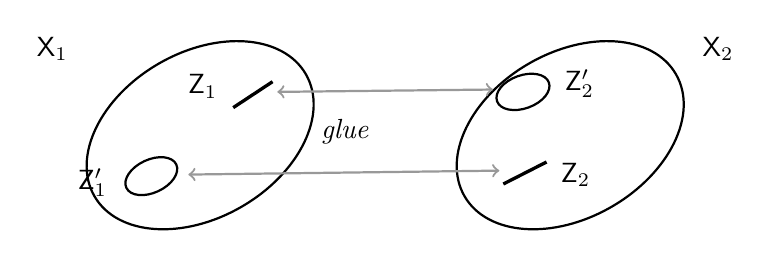
\begin{tikzpicture}[line width=0.8pt]
  \draw[rotate around={30:(0,0)}] (0,0) ellipse (1.55 and 1.05);
  \draw[rotate around={30:(4.7,0)}] (4.7,0) ellipse (1.55 and 1.05);
  \draw[line width=1.2pt] (0.42,0.35) -- (0.92,0.68);
  \node[anchor=east] at (0.35,0.62) {$\mathsf{Z}_1$};
  \draw[rotate around={25:(-0.62,-0.52)}] (-0.62,-0.52) ellipse (0.35 and 0.21);
  \node[anchor=east] at (-1.05,-0.6) {$\mathsf{Z}'_1$};
  \draw[rotate around={20:(4.1,0.55)}] (4.1,0.55) ellipse (0.35 and 0.21);
  \node[anchor=west] at (4.5,0.66) {$\mathsf{Z}'_2$};
  \draw[line width=1.2pt] (3.85,-0.62) -- (4.4,-0.34);
  \node[anchor=west] at (4.45,-0.5) {$\mathsf{Z}_2$};
  \node[anchor=east] at (-1.55,1.1) {$\mathsf{X}_1$};
  \node[anchor=west] at (6.25,1.1) {$\mathsf{X}_2$};
  \draw[gray!80,<->] (0.98,0.55) -- (3.72,0.58);
  \draw[gray!80,<->] (3.8,-0.45) -- (-0.15,-0.5);
  \node at (1.85,0.05) {\textit{glue}};
\end{tikzpicture}
\caption{搭建一个\trProper{}的非射影\trVariety。（依原书手绘图重绘。）}\label{fig:proper-nonprojective-variety}
\end{figure}

那么 $X$ 不是射影的。因为若它是，则它将经由某个\trInvertibleSheaf{} $\mathscr{L}$ 嵌入\trProjectiveSpace。若 $X$ 被嵌入，则 $X_1$ 也被嵌入，于是 $\mathscr{L}$ 限制到 $X_1$ 上必是形如 $\OO_{X_1}(n_1)$ 的\trInvertibleSheaf，其中 $n_1>0$。你可以验证：$\mathscr{L}$ 限制到 $Z_1$ 上是 $\OO_{Z_1}(n_1)$，而 $\mathscr{L}$ 限制到 $Z'_1$ 上是 $\OO_{Z'_1}(2n_1)$。对称地，$\mathscr{L}$ 限制到 $Z_2$ 上是 $\OO_{Z_2}(n_2)$，对某个 $n_2>0$，而 $\mathscr{L}$ 限制到 $Z'_2$ 上是 $\OO_{Z'_2}(2n_2)$。但粘合之后，$Z_1=Z'_2$，且 $Z'_1=Z_2$，于是我们有 $n_1=2n_2$ 与 $2n_1=n_2$，这是不可能的。

\textbf{15.2.12.}\ \emph{沿\trIsomorphic{}的\trClosedSubscheme{}粘合两个\trScheme。}

直截了当地证明：你可以沿\trIsomorphic{}的\trOpenSubscheme{}粘合两个\trScheme。（更精确地说，若 $X_1$ 与 $X_2$ 是\trScheme，分别带有\trOpenSubscheme{} $U_1$ 与 $U_2$，以及一个\trIsomorphism{} $U_1\overset{\sim}{\hookrightarrow}U_2$，那么你可以对「沿 $U_1\overset{\sim}{\hookrightarrow}U_2$ 粘合 $X_1$ 与 $X_2$」讲得通。你应当把这件事想清楚。）类似地，你也可以沿\trIsomorphic{}的\emph{闭}子概形粘合两个\trScheme。我们现在把这件事说精确。设 $Z_1\hookrightarrow X_1$ 与 $Z_2\hookrightarrow X_2$ 是\trClosedEmbedding，而
\[
\phi\colon Z_1\overset{\sim}{\longrightarrow}Z_2
\]
是一个\trIsomorphism。我们将解释如何沿 $\phi$ 把 $X_1$ 粘合到 $X_2$ 上。其结果将被称为 $X_1\amalg_\phi X_2$。

\textbf{15.2.13.}\ \emph{动机示例。}\quad 我们的动机示例是：若 $X_i=\Spec A_i$，$Z_i=\Spec A_i/I_i$，而 $\phi$ 对应于 $\phi^{\sharp}\colon A_2/I_2\overset{\sim}{\longrightarrow}A_1/I_1$。那么其结果将是 $\Spec R$，其中 $R$ 是由那些「经由 $\phi$ 相合」的有序对 $(a_1,a_2)\in A_1\times A_2$ 组成的\trRing。更精确地说，这是一个环的\trFiberProduct：
\[
R:=A_1\times_{\phi^{\sharp}\colon A_1/I_1\to A_2/I_2}A_2.
\]

\textbf{15.2.14.}\ \emph{一般构造，作为一个\trLocallyRingedSpace。}\quad 在我们的一般情势下，我们或许希望用这种形式的开片盖住 $X_1$ 与 $X_2$。那样我们将不得不为粘合与选取而操心，所以为了避免这些，我们改为先把 $X_1\amalg_\phi X_2$ 作为一个\trLocallyRingedSpace{}构造出来。作为一个\trTopologicalSpace，其定义是清楚的：把二者的\trUnderlyingSet{}沿着 $Z_1\cong Z_2$ 的\trUnderlyingSet{}粘合起来，并给这个粘合而成的集合赋予\trTopology，使得 $X_1\amalg_\phi X_2$ 的一个子集是\trOpen{}的，当且仅当它限制到 $X_1$ 与 $X_2$ 上都是\trOpen{}的。为方便起见，令 $Z$ 为 $Z_1$（或者，等价地，$Z_2$）在 $X_1\amalg_\phi X_2$ 中的\trImage。接下来，我们在每个点 $p\in X_1\amalg_\phi X_2$ 处定义\trStructureSheaf{}的\trStalk。若 $p\in X_i\setminus Z=(X_1\amalg_\phi X_2)\setminus X_{3-i}$（希望这一点含义是清楚的），我们便把\trStalk{}定义为 $\OO_{X_i,p}$。若 $p\in X_1\cap X_2$，我们把\trStalk{}定义为由那些在 $\OO_{Z_1,p}\cong\OO_{Z_2,p}$ 中相合的元素 $(s_1,s_2)\in\OO_{X_1,p}\times\OO_{X_2,p}$ 组成。如果你能完成下面这道练习，本段中一切的含义对你来说都会是清楚的。

\textbf{15.2.J.（练习）}\quad 用\trCompatibleGerm{}定义 $\OO_{X_1\amalg_\phi X_2}$ 的\trStructureSheaf。（芽\trCompatible{}应当是什么意思？提示：对 $z\in Z$，设我们有 $X_1$ 的\trOpenSubset{} $U_1$ 与 $X_2$ 的\trOpenSubset{} $U_2$，满足 $U_1\cap Z=U_2\cap Z$，于是 $U_1$ 与 $U_2$ 粘合起来给出 $X_1\amalg_\phi X_2$ 的一个\trOpenSubset{} $U$。又设我们在 $U_1$ 上有函数 $f_1$、在 $U_2$ 上有函数 $f_2$，它们「在 $U\cap Z$ 上相合」——这是什么意思？那么我们就宣称：「把 $f_1$ 与 $f_2$ 粘合起来而在 $U$ 上得到的函数」的诸\trGerm{}是\trCompatible{}的。）证明：所得到的\trRingedSpace{}是一个\trLocallyRingedSpace。

接下来我们想证明：\trLocallyRingedSpace{} $X_1\amalg_\phi X_2$ 是一个\trScheme。显然它在远离 $Z$ 处是一个\trScheme。我们先验证一个特例。

\textbf{15.2.K.（练习）}\quad 证明：在\mbox{例~15.2.13} 中，\S15.2.14 的构造确实给出 $\Spec(A_1\times_{\phi^{\sharp}}A_2)$。

\textbf{15.2.L.（练习）}\quad 在一般情形，设 $x\in Z$。证明：存在一个\trAffine\trOpenSubset{} $\Spec A_1\subset X_1$，使得 $Z\cap\Spec A_1=Z\cap\Spec A_2$。然后用\mbox{练习~15.2.J} 证明：$X_1\amalg_\phi X_2$ 在 $x$ 的一个\trOpen\trNeighborhood{}中是一个\trScheme，从而是一个\trScheme。

\textbf{15.2.15.}\ \emph{\trhRemark{}。}

（a）正如记号所暗示的，这是\trScheme{}的\trCategory{}中的一个\trFiberedCoproduct，而且实际上在\trLocallyRingedSpace{}的\trCategory{}中也是如此。我们并不需要这个事实，但你若愿意可以证明它；这并不难。与积的情状不同，\trFiberedCoproduct{}在\trScheme{}的\trCategory{}中一般并不存在。神奇的是（并且出于对\trScheme{}而言特殊的原因），所得的余纤维图表同时也是一个\emph{纤维}（fibered，即\trCartesianDiagram）图表。这有令人愉快的推论。例如，这个构造「对平坦\trBaseChange{}表现良好」（或者说与平坦\trBaseChange{}「交换」）。

（b）你或许会希望：若你有一个\trScheme{} $X$，带着两个不相交的\trClosedSubscheme{} $W'$ 与 $W''$，以及一个\trIsomorphism{} $W'\overset{\sim}{\longrightarrow}W''$，那么你应当能够沿 $W'\to W''$ 把 $X$ 与自身粘合起来。这个构造行不通，而且的确可能根本办不到。你仍然可以把这个商作为一个\trAlgebraicSpace{}来讲得通，我们不打算在这里定义它。

\textbf{15.2.M.（练习）}\quad 我们继续使用记号 $X_i$、$\phi$ 等等。设我们在 $A$-\trScheme{}的\trCategory{}中工作。

（a）若 $X_1$ 与 $X_2$ 都是\trUniversallyClosed{}的，证明 $X_1\amalg_\phi X_2$ 亦然。

（b）若 $X_1$ 与 $X_2$ 都是\trSeparated{}的，证明 $X_1\amalg_\phi X_2$ 亦然。

（c）若 $X_1$ 与 $X_2$ 都是在\trNoether\trRing{} $A$ 上\trFiniteType{}的，证明 $X_1\amalg_\phi X_2$ 亦然。（提示：化归到\mbox{动机示例~15.2.13} 的「\trAffine」情形。选取 $A_1$ 的\trGenerator{} $x_1,\dots,x_n$ 与 $y_1,\dots,y_n$，使得经由 $\phi$，$x_i$ 模 $I_1$ 与 $y_i$ 模 $I_2$ 相合。选取 $I_2$ 的\trGenerator{} $g_1,\dots,g_m$——这里要用到 $A$ 的诺特性。证明 $(x_i,y_i)$ 与 $(0,g_i)$ 生成 $R\subset A_1\times A_2$，如下。设 $(a_1,a_2)\in R$\footnote{原书此处作「$(a,b)\in(A,B)$」，其中 $(A,B)$ 当系 $A\times B$ 之误（该二元组系 $R\subset A_1\times A_2$ 中元素），径改。——译者注}。那么存在某个多项式 $m$ 使得 $a_1=m(x_1,\dots,x_n)$。于是对某个 $a'_2\in I_2$，$(a_1,a_2)-m((x_1,y_1),\dots,(x_n,y_n))=(0,a'_2)$。而这个 $a'_2$ 可以写成 $\sum_{i=1}^m\ell_i(y_1,\dots,y_n)g_i$。但随后 $(0,a'_2)=\sum_{i=1}^m\ell_i((x_1,y_1),\dots,(x_n,y_n))(0,g_i)$。）

于是若 $X_1$ 与 $X_2$ 都是\trProper{}的，则 $X_1\amalg_\phi X_2$ 亦然。

另一方面，我们刚刚看到（\S15.2.11）：若 $X_1$ 与 $X_2$ 都是\emph{射影}的，则 $X_1\amalg_\phi X_2$ 未必射影。

\textbf{15.2.16.}\ \emph{玩转更一般的概形「粘合」（\trCoproduct）。}\quad 若你读到了这里，你就可以相当廉价地看到更多有意思的例子。设更一般地，你有一个\trClosedEmbedding{} $Z\hookrightarrow Y$，而只有一个\trAffine\trMorphism{} $Z\to X$。我们仍然可以沿 $Z$ 把 $X$ 与 $Y$「粘合」起来得到一个\trScheme{} $W$，做法是遵循同一个配方。

\textbf{15.2.N.（扩展练习）}\quad 给定一个\trClosedEmbedding{} $\alpha\colon Z\hookrightarrow X$ 与一个\trAffine\trMorphism{} $\beta\colon Z\to Y$，证明（遵循 \S15.2.12 的策略）：存在一张概形的\trFiberedCoproduct{}方图
\begin{equation*}\tag{15.2.16.1}\label{eq:pushout-square-schemes}
\begin{tikzcd}[column sep=3.5em, row sep=3.5em]
Z \ar[r, "\beta\;\text{仿射}"] \ar[d, hook, "\alpha\;\text{闭嵌入}"] & Y \ar[d, "\alpha'"'] \\
X \ar[r, "\beta'"] & W.
\end{tikzcd}
\end{equation*}
这张方图在相差唯一\trIsomorphism{}的意义下必然唯一。

\textbf{15.2.O.（练习）}\quad 证明：\eqref{eq:pushout-square-schemes} 同时也是一个拉回方图（即\trCartesianDiagram），并且 $\alpha'$ 是一个\trClosedEmbedding，$\beta'$ 是一个\trAffine\trMorphism。

\textbf{15.2.17.}\ \emph{一个没有\trClosedPoint{}的\trScheme。}

在求解\mbox{扩展练习~15.2.N} 的过程中，你将会研究那个（容易得多的）\trAffine{}情形，它对应于下面这张环的方图。
\begin{equation*}\tag{15.2.17.1}\label{eq:pushout-square-rings}
\begin{tikzcd}[column sep=4.5em, row sep=3.5em]
A/I & B \ar[l, "\beta^{\sharp}"] \\
A \ar[u] & A\times_{A/I}B \ar[l] \ar[u]
\end{tikzcd}
\end{equation*}

于是对应于 $W$ 的那个环可以被解读为
\[
A\times_{A/I}B=\{(a,b)\in A\times B : a\equiv\alpha^{\sharp}(b)\pmod{I}\}.
\]

我们可以用这个构造来看到一些有意思的行为。例如，我们现在来描述一个没有\trClosedPoint{}的\trScheme{} $X$。它将有可数多个点 $\{p_1,p_2,\dots\}$，而它的诸\trOpenSet{}将形如 $\{p_1,\dots,p_n\}$。（显然这个\trTopologicalSpace{}没有\trClosedPoint{}。）每个\trOpenSet{}都将是\trAffine{}的：$\{p_1,\dots,p_n\}=\Spec A_n$。我们如下归纳地构造 $A_n$。令 $A_1=k(x_1,x_2,\dots)$（\trField{} $k$ 的一个可数生成超越扩张）。我们归纳地构造 $A_{n+1}$，用的是 \eqref{eq:pushout-square-rings} 的如下特例：
\[
\begin{tikzcd}[column sep=7.5em, row sep=3.5em]
k(x_n,x_{n+1},\dots) & k(x_{n+1},x_{n+2},\dots)[x_n]_{x_n} \ar[l, hook] \\
A_n \ar[u] & A_{n+1} \ar[l, hook] \ar[u]
\end{tikzcd}
\]
顶上一行不过是一个\trDVR{}映入其\trFractionField{} $K$。左面一列是一个复杂的\trLocalRing，其\trResidueField{}正是同一个域 $K$。

把注意力集中在 $\{p_1,p_2,p_3\}$ 上时，这件事可能更容易理解。令 $F=k(x_3,x_4,\dots)$。那么 $A_1$ 是一个\trField，$A_2$ 是\trDVR{} $F(x_2)[x_1]_{x_1}$，而 $A_3$ 是 $A_2$ 的一个\trSubring，其模 $x_1$ 的剩余落在\trDVR{} $F[x_2]_{x_2}$ 之中。（环 $A_3$ 是一个\emph{\trRank{} $2$ \trValuationRing}的例子；你能看出它为何配得上这个名字吗？）

\textbf{15.2.P.（练习）}\quad 利用上述内容描述一个没有\trClosedPoint{}的\trScheme{} $\bigcup_{n\ge 1}\Spec A_n$。

